% !TeX encoding = UTF-8
% !TeX spellcheck = es_ES
\documentclass[12pt]{article}
\usepackage{fullpage}
\usepackage[utf8]{inputenc}
\usepackage{pict2e}
\usepackage{amsmath}
\usepackage{enumitem}
\usepackage{eurosym}
\usepackage{mathtools}
\usepackage{amssymb, amsfonts, latexsym, cancel}
\setlength{\parskip}{0.3cm}
\usepackage{graphicx}
\usepackage{fontenc}
\usepackage{setspace}
\usepackage{adjustbox}
\usepackage{float}
\setstretch{1.35}
\usepackage{bold-extra}
\usepackage{subcaption}
\pagestyle{empty}
\graphicspath{ {images/} }
\usepackage{tcolorbox}
\usepackage{xcolor, colortbl}
\usepackage{wrapfig}
\usepackage{empheq}
\usepackage{array}
\usepackage{parskip}
\usepackage{arydshln}
\renewcommand*\contentsname{\color{black}Índice} 
\usepackage{array, multirow, multicol}
\definecolor{lightblue}{HTML}{007AFF}
\usepackage{color}
\usepackage{etoolbox}
\usepackage{listings}
\usepackage{mdframed}
\setlength{\parindent}{0pt}
\usepackage{underscore}
\usepackage{hyperref}
\usepackage{tikz}
\usetikzlibrary{shapes, positioning, patterns}
\usepackage{tikz-qtree}
\usepackage{biblatex}
\usepackage{pdfpages}
\usepackage{pgfplots}
\usepackage{pgfkeys}
\usepackage{mathrsfs}
\addbibresource{biblatex-examples.bib}
\usepackage[a4paper, left=1cm, right=1cm, top=1cm,
bottom=1.5cm]{geometry}
\everymath{\displaystyle}
\usetikzlibrary{decorations.pathreplacing, calc}
\usepackage{titlesec}
\usepackage{pgffor}
\usepackage{subcaption}
\setlength{\fboxrule}{1.5pt}
\renewcommand{\arraystretch}{1.2}

% Configura el formato de las secciones utilizando titlesec
\titleformat{\section}
{\color{red}\normalfont\LARGE\bfseries}
{Tema \thesection:}
{10 pt}
{}

\titleformat{\subsection}
{\normalfont\Large\bfseries\color{red}}{\thesubsection)}{1em}{\color{lightblue}}

\titleformat{\subsubsection}
{\normalfont\large\bfseries\color{red}}{\thesubsubsection)}{1em}{\color{lightblue}}

\newcommand{\bboxed}[1]{\fcolorbox{lightblue}{lightblue!10}{$#1$}}
\newcommand{\rboxed}[1]{\fcolorbox{red}{red!10}{$#1$}}

\newcommand{\bu}[1]{\textcolor{lightblue}{\underline{#1}}}
\newcommand{\lb}[1]{\textcolor{lightblue}{#1}}
\newcommand{\db}[1]{\textcolor{blue}{#1}}
\newcommand{\rc}[1]{\textcolor{red}{#1}}

\newcommand{\dx}{\:\mathrm{d}x}
\newcommand{\dt}{\:\mathrm{d}t}
\newcommand{\dy}{\:\mathrm{d}y}
\newcommand{\dz}{\:\mathrm{d}z}
\newcommand{\dth}{\:\mathrm{d}\theta}
\newcommand{\dr}{\:\mathrm{d}\rho}
\newcommand{\du}{\:\mathrm{d}u}
\newcommand{\dv}{\:\mathrm{d}v}
\newcommand{\tozero}[1]{\cancelto{0}{#1}}
\newcommand{\lbb}[2]{\textcolor{lightblue}{\underbracket[1pt]{\textcolor{black}{#1}}_{#2}}}
\newcommand{\dbb}[2]{\textcolor{blue}{\underbracket[1pt]{\textcolor{black}{#1}}_{#2}}}
\newcommand{\rb}[2]{\textcolor{red}{\underbracket[1pt]{\textcolor{black}{#1}}_{#2}}}
\DeclareMathOperator{\N}{\mathbb{N}}
\DeclareMathOperator{\Z}{\mathbb{Z}}
\DeclareMathOperator{\R}{\mathbb{R}}
\DeclareMathOperator{\Q}{\mathbb{Q}}
\DeclareMathOperator{\K}{\mathbb{K}}

\renewcommand{\CancelColor}{\color{lightblue}}

\begin{document}
\begin{enumerate}[label=\color{red}\textbf{\arabic*)}, leftmargin=*]
\item \lb{Calcula las siguientes integrales (utiliza integración por partes):}

$\db{\int\ln(x)\dx=}\int1\cdot\ln(x)\dx=\left\{\begin{array}{ll}
      u=\ln(x) & \du=\dfrac{1}{x}\dx\\
      \dv=1\dx & v=x
\end{array}\right\}=x\ln(x)-\int x\cdot\dfrac{1}{x}\dx=x\ln(x)-\int1\dx=\bboxed{x\ln(x)-x+\mathrm{C}}$
\item \lb{Calcula las siguientes integrales (utiliza integración por partes):}

$\begin{aligned}
      \db{\textcolor{lightblue}{\underbracket[1pt]{\textcolor{blue}{\int\sin(2x)e^{4x}}}_{I}}}&=\left\{\begin{array}{ll}
      u=\sin(2x) & \du=2\cos(2x)\dx\\
      dv=e^{4x}\dx& v=\dfrac{e^{4x}}{4}
\end{array}\right\}=\dfrac{1}{4}e^{4x}\sin(2x)-\dfrac{1}{2}\int e^{4x}\cos(2x)\dx\\
&=\left\{\begin{array}{ll}
u=\sin(2x) & \du=2\cos(2x)\dx\\
dv=e^{4x}\dx& v=\dfrac{e^{4x}}{4}
\end{array}\right\}\\
&=-\dfrac{1}{4}e^{4x}\sin(2x)-\dfrac{1}{2}\left(\dfrac{1}{4}e^{4x}\sin(2x)-\dfrac{1}{2}\int e^{4x}\cos(2x)\dx\right)\\
&=\dfrac{1}{4}e^{4x}\sin(2x)-\dfrac{1}{8}e^{4x}\cos(2x)-\dfrac{1}{4}\lbb{\int e^{4x}\sin(2x)\dx}{I}
\end{aligned}$

Podemos escribir esto como: \[ \begin{array}{l}
      I=\dfrac{1}{4}e^{4x}\sin(2x)-\dfrac{1}{8}e^{4x}\cos(2x)-\dfrac{1}{4}I\longrightarrow \dfrac{5}{4}I=\dfrac{1}{4}e^{4x}\sin(2x)-\dfrac{1}{8}e^{4x}\cos(2x)\\
      \\
      \bboxed{I=\dfrac{1}{5}e^{4x}\sin(2x)-\dfrac{1}{10}e^{4x}\cos(2x)+\mathrm{C}}
\end{array} \]
\item \lb{Calcula las siguientes integrales (utiliza integración por partes):}

$\db{\int x^2e^{2x}\dx=}\left\{\begin{array}{ll}
      u=x^2 & \du=2x\dx\\
      \dv=e^{2x}\dx & v=\dfrac{e^{2x}}{2}
\end{array}\right\}=\dfrac{1}{2}x^2e^{2x}-\int xe^{2x}\dx=\left\{\begin{array}{ll}
u=x^2 & \du=2x\dx\\
\dv=e^{2x}\dx & v=\dfrac{e^{2x}}{2}
\end{array}\right\}=\dfrac{1}{2}x^2e^{2x}-\left(\dfrac{1}{2}xe^{x^2}-\int\dfrac{1}{2}e^{2x}\dx\right)=\dfrac{1}{2}x^2e^{2x}-\dfrac{1}{2}xe^{2x}+\dfrac{1}{2}\int e^{2x}\dx=\bboxed{\dfrac{1}{2}x^2ex^{2x}-\dfrac{1}{2}xe^{2x}+\dfrac{1}{4}e^{2x}+\mathrm{C}}$
\item \lb{Calcular las primitivas de las siguientes fracciones racionales:}

$\db{\int\dfrac{x^7+x^3}{x^4-1}\dx}$

Como el polinomio del numerador es de grado mayor que es del denominador, dividiremos los polinomios y aplicaremos el algoritmo de Euclides: $\dfrac{N(x)}{D(x)}=C(x)+\dfrac{R(x)}{D(x)}$

\begin{tabular}{rl}
      $x^7+x^3$ & \multicolumn{1}{|l}{$x^4-1$}\\ \cline{2-2}
      $-x^7+x^3$ & $x^3$ \\ \cline{1-1}
      $2x^3$
\end{tabular}$\longrightarrow\dfrac{x^7+x^3}{x^4-1}=x^3+\dfrac{2x^3}{x^4-1}$

$\begin{array}{l}
      \int\dfrac{x^7+x^3}{x^4-1}\dx=\int x^3+\dfrac{2x^3}{x^4-1}\dx=\int x^3\dx+\lbb{\int\dfrac{2x^3}{x^4-1}}{I}=\bboxed{\dfrac{x^4}{4}+\dfrac{1}{2}\log|x^4-1|+\mathrm{C}}\\
      \lb{I=}\int\dfrac{2x^3}{x^4-1}\dx=\dfrac{1}{2}\int\dfrac{4x^3}{x^4-1}\dx=\left\{\begin{array}{l}
            x^4-1=t\\
            4x^3\dx=\dt
      \end{array}\right\}=\dfrac{1}{2}\int\dfrac{1}{t}\dt=\dfrac{1}{2}\log(t)=\dfrac{1}{2}\log|x^4-1|
\end{array}$
\item \lb{Calcular las primitivas}

$\db{\int\cos(x)^4\sin(x)^3\dx=}\int\cos^4(x)\cdot\sin^2(x)\cdot\sin(x)\dx=\int\cos^4(x)(1-\cos^2(x))\sin(x)\dx=-\int\cos^4(x)(1-\cos^2(x))(-\sin(x))\dx=\left\{\begin{array}{l}
      \cos(x)=t\\
      -\sin(x)\dx=\dt
\end{array}\right\}=-\int t^4\cdot(1-t^2)\dt=-\int t^4-t^6\dt=-\dfrac{t^5}{5}+\dfrac{t^7}{7}+\mathrm{C}=\bboxed{-\dfrac{\cos^5(x)}{5}+\dfrac{\cos^7(x)}{7}+\mathrm{C}}$
\item \lb{Calcular las siguientes integrales definidas:}

$\db{\int_{0}^{1}xe^{x}\dx}$

\begin{minipage}[l]{\textwidth}
      \begin{wrapfigure}[4]{r}{0.35\textwidth}
            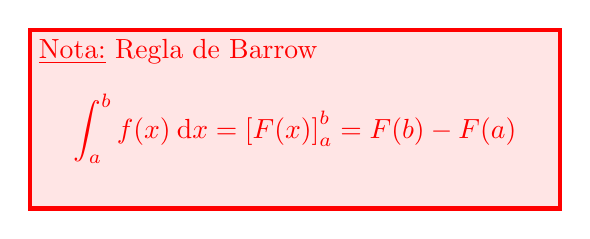
\begin{tikzpicture}[baseline=(current bounding box.center)]
                  \node[red,draw=red,fill=red!10,line width=1.5pt,text width=6.5cm] {\underline{Nota:} Regla de Barrow \[ \int_{a}^{b}f(x)\dx=\left[F(x)\right]_a^b=F(b)-F(a) \]};
            \end{tikzpicture}
      \end{wrapfigure}
      
      Calcularemos lo primero la primitiva: \[ \int xe^{x}\dx=\left\{\begin{array}{ll}
            u=x & \du=\dx\\
            \dv=e^{x}\dx & v=e^x
      \end{array}\right\}=xe^{x}-\int e^x\dx=xe^x-e^x \]Evaluando en la integral definida tenemos que: \[ \int_{0}^{1}xe^x\dx=\left[xe^x-e^x\right]_0^1=\left(\cancel{e}-\cancel{e}\right)-(0-1)=\bboxed{1} \]
\end{minipage}
\item \lb{Calcular las siguientes integrales definidas:}

$\db{\int_{0}^{\frac{\pi}{2}}\sin(x)\dx=}\left[-\cos(x)\right]_0^{\frac{\pi}{2}}=\tozero{-\cos\left(\dfrac{\pi}{2}\right)}+1=\bboxed{1}$

\item \lb{Calcula mediante cambio de variable:}

\begin{minipage}[l]{\textwidth}
      \begin{wrapfigure}{r}{0.5\textwidth}
            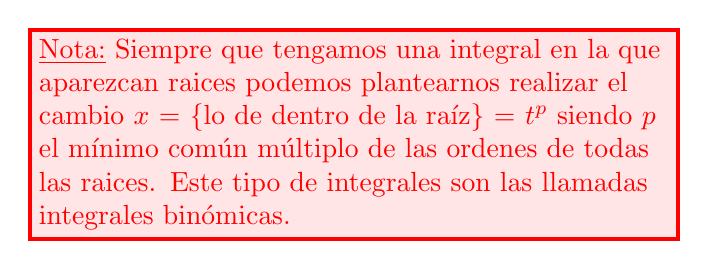
\begin{tikzpicture}[baseline=(current bounding box.center)]
                  \node[red,draw=red,fill=red!10,line width=1.5pt,text width=8cm] {\underline{Nota:} Siempre que tengamos una integral en la que aparezcan raices podemos plantearnos realizar el cambio $x=\{\text{lo de dentro de la raíz}\}=t^p$ siendo $p$ el mínimo común múltiplo de las ordenes de todas las raices. Este tipo de integrales son las llamadas integrales binómicas.};
            \end{tikzpicture}
      \end{wrapfigure}
      
      $\db{\int\dfrac{\dx}{x+\sqrt{x}}}$
      
      $\int\dfrac{1}{x+\sqrt{x}}\dx=\left\{\begin{array}{l}
            x=t^2\\
            \dx=2t\dt
      \end{array}\right\}=\int\dfrac{1}{t^2+t}\cdot2t\dt=\int\dfrac{2\cancel{t}}{\cancel{t}(t+1)}\dt=2\int\dfrac{1}{t+1}\dt=2\log|x+1|+\mathrm{C}=\bboxed{2\log(\sqrt{x}+1)+\mathrm{C}}$
\end{minipage}
\item \lb{Calcula mediante cambio de variable:}

$\db{\int\dfrac{x^2}{\sqrt{x+a}}\dx=}\left\{\begin{array}{l}
      x+a=t^2\\
      x=t^2-a\\
      \dx=2t\dt
\end{array}\right\}=\int\dfrac{(t^2-a)^2}{\cancel{t}}\cdot 2\cancel{t}\dt=2\int t^4+a^2-2at^2\dt=2\left[\dfrac{t^5}{5}+a^2t-2a\cdot\dfrac{t^3}{3}\right]=\bboxed{\dfrac{2}{5}\left(\sqrt{x+a}\right)^5+2a^2\sqrt{x+a}-\dfrac{4}{3}a\left(\sqrt{x+a}\right)^3+\mathrm{C}}$
\item \lb{Calcular la siguiente integral:}

$\begin{array}{l}
      \db{\int\dfrac{1}{\sqrt{x}+\sqrt[3]{x}}\dx=}\left\{\begin{array}{l}
            x=t^6\\
            \dx=6t^5\dt
      \end{array}\right\}=\int\dfrac{1}{t^3+t^2}\cdot6^5\dt=\int\dfrac{6t^{\cancel{5}}}{\cancel{t^2}(t+1)}\dt=\int\dfrac{6t^3}{t+1}=\lb{(\ast)}\\
      \begin{array}{rrrrl}
            6t^3 &  &  &  & \multicolumn{1}{|l}{t+1} \\ \cline{5-5}
            -6t^3 & -6t^2 &  &  & 6t^2-6t+6 \\ \cline{1-2}
            &  -6t^2 &  &  &  \\
            & 6t^2 & +6t  &  &  \\ \cline{2-3}
            &  & 6t  &  &  \\
            &  & -6t & -6 &  \\ \cline{3-4}
            &  &  & -6 & 
      \end{array} \qquad\bboxed{\dfrac{6t^3}{t+1}=6t^2-6t+6-\dfrac{6}{t+1}}\\
      \begin{aligned}
            \lb{(\ast)=}\int6t^2-6t+6-\dfrac{6}{t+1}\dt&=\dfrac{6t^3}{3}-\dfrac{6t^2}{2}+6t-6\ln|t+1|+\mathrm{C}=2t^3-3t^2+6t-6\ln|t+1|+\mathrm{C}\\
             &=2(\sqrt[6]{x})^3-3(\sqrt[6]{x})^2+6\sqrt[6]{x}-6\ln|\sqrt[6]{x}+1|+\mathrm{C}\\
             &=\bboxed{2\sqrt{x}-3\sqrt[3]{x}+6\sqrt[6]{x}-6\ln(\sqrt[6]{x}+1)+\mathrm{C}}
      \end{aligned}
\end{array}$
\item \lb{Halle las derivadas de cada una de las siguientes funciones:}

\begin{minipage}[l]{\textwidth}
      \begin{wrapfigure}{r}{0.5\textwidth}
            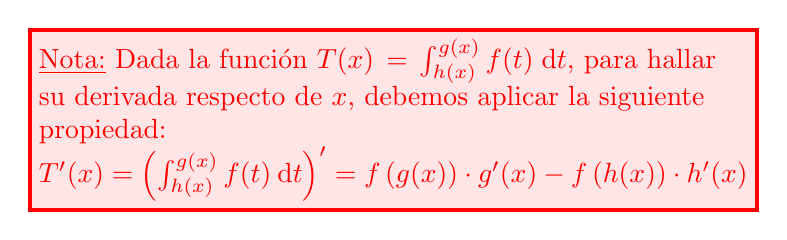
\begin{tikzpicture}[baseline=(current bounding box.center)]
                  \node[red,draw=red,fill=red!10,line width=1.5pt,text width=9cm] {\underline{Nota:} Dada la función $T(x)=\int_{h(x)}^{g(x)}f(t)\dt$, para hallar su derivada respecto de $x$, debemos aplicar la siguiente propiedad: 
                        
                        $T'(x)=\left(\int_{h(x)}^{g(x)}f(t)\dt\right)'=f\left(g(x)\right)\cdot g'(x)-f\left(h(x)\right)\cdot h'(x) $};
            \end{tikzpicture}
      \end{wrapfigure}
      
      $\db{F(x)=\int_{a}^{x^3}\sin^3(t)\dt}$
      
      $F'(x)=\left(\int_{a}^{x^3}\sin^3(t)\dt\right)'=\sin^3(x^3)\cdot3x^2-\sin^3(a)\cdot0\longrightarrow\bboxed{F'(x)=3x^2\cdot\sin^3(x^3)}$
\end{minipage}

\vspace{2cm}

\item \lb{Calcula:}

$\begin{array}{l}
      \begin{aligned}
            \db{\lim_{x\to0^+}\dfrac{\int_{0}^{x^2}\sin(\sqrt{t})\dt}{x^3}=}\left(\dfrac{0}{0}\right)&=\{\text{L'Hôpital}\}=\lim_{x\to0^+}\dfrac{2\cancel{x}\sin(x)}{3x^{\cancel{2}}}=\lim_{x\to0^+}\dfrac{2\sin(x)}{3x}=\left(\dfrac{0}{0}\right)\\
            &=\left\{\begin{array}{l}
      \text{equivalencias}\\
      \sin(x)\leadsto_0x
\end{array}\right\}=\lim_{x\to0^+}\dfrac{2x}{2x}=\bboxed{\dfrac{2}{3}}
      \end{aligned}\\
\left(\int_{0}^{x^2}\sin(\sqrt{t})\dt\right)'=\sin(x)\cdot 2x-\cancel{\sin(0)\cdot0}=2x\sin(x)
\end{array}$
\item \lb{Calcular las siguientes integrales definidas:}

$\db{\int_{1}^{2}\log(x)\dx}$

Empezamos calculando la primitiva, para luego poder sustituirla: \[ \int1\log(x)\dx=\left\{\begin{array}{ll}
      u=\log(x) & \du=\dfrac{1}{x}\dx\\
      \dv=1\dx & v=x
\end{array}\right\}=x\log(x)-\int x\cdot\dfrac{1}{x}\dx=x\log(x)-\int1\dx=x\log(x)-x \]Una vez que tenemos la primitiva, evaluamos: \[ \int_{1}^{2}\log(x)\dx=\left[x\log(x)-x\right]_1^2=\left(2\log(2)-2\right) -(\tozero{\log(1)}-1)=\bboxed{2\log(2)-1}\]

\item \lb{Calcular las siguientes integrales}

$\db{\int\dfrac{1}{x\sqrt{1-\ln^2(x)}}\dx=}\int\dfrac{1}{x}\cdot\dfrac{1}{\sqrt{1-\ln^2(x)}}\dx=\left\{\begin{array}{l}
      \ln(x)=t\\
      \dfrac{1}{x}\dx=\dt
\end{array}\right\}=\int\dfrac{1}{\sqrt{1-t^2}}\dt=\arcsin(t)=\bboxed{\arcsin(\ln(x))+\mathrm{C}}$

\item \lb{Calcular las siguientes integrales definidas:}

$\db{\int_{0}^{3}\dfrac{x}{\sqrt{x+1}}\dx}$

Comenzaremos calculando la primera, para luego poder evaluar: 

$ \int\dfrac{x}{\sqrt{x+1}}\dx=\left\{\begin{array}{l}
      x+1=t^2\\
      x=t^2-1\\
      \dx=2t\dt
\end{array}\right\}=\int\dfrac{t^2-1}{\cancel{t}}\cdot2\cancel{t}\dt=2\int t^2-1\dt=2\left[\dfrac{t^3}{3}-t\right]=\{t=\sqrt{x+1}\}=\dfrac{2}{3}(\sqrt{x+1})^3-2\sqrt{x+1} $

Evaluar tenemos que: \[ \int_{0}^{3}\dfrac{x}{\sqrt{x+1}}\dx=\left[\dfrac{2}{3}(\sqrt{x+1})^3-2\sqrt{x+1}\right]_{0}^{3}0\left(\dfrac{2}{3}8-4\right)-\left(\dfrac{2}{3}-2\right)=\dfrac{16}{3}-\dfrac{12}{3}-\dfrac{2}{3}+\dfrac{6}{3}=\bboxed{\dfrac{8}{3}} \]
\item \lb{Halle $F'(x)$ si $F(x)=\int_{0}^{x}xf(t)\dt$}

\begin{minipage}[l]{\textwidth}
      \begin{wrapfigure}{r}{0.45\textwidth}
            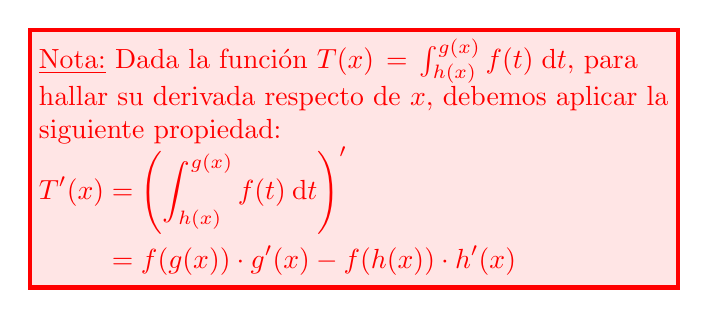
\begin{tikzpicture}[baseline=(current bounding box.center)]
                  \node[red,draw=red,fill=red!10,line width=1.5pt,text width=8cm] {\underline{Nota:} Dada la función $T(x)=\int_{h(x)}^{g(x)}f(t)\dt$, para hallar su derivada respecto de $x$, debemos aplicar la siguiente propiedad: 
                        
                        $ \begin{aligned}
                              T'(x)&=\left(\int_{h(x)}^{g(x)}f(t)\dt\right)'\\
                              &=f(g(x))\cdot g'(x)-f(h(x))\cdot h'(x)
                        \end{aligned}$};
            \end{tikzpicture}
      \end{wrapfigure}
      
      $F(x)=\int_{0}^{x}xf(t)\dt=\lbb{x}{}\cdot\lbb{\int_{0}^{x}f(t)\dt}{}$
      
      $F'(x)=\{\text{derivada de un producto}\}=1\cdot\int_{0}^{x}f(t)\dt+x\left(\int_{0}^{x}f(t)\dt\right)'=\int_{0}^{x}f(t)\dt+x\left[f(x)\cdot1-\tozero{f(0)\cdot0}\right]=\int_{0}^{x}f(t)\dt+x\cdot f(x)$
      
      Por lo tanto: $\bboxed{F'(x)=\int_{0}^{x}f(t)\dt+xf(x)}$
\end{minipage}

\item \lb{Calcular las siguientes integrales}

$\db{\int\dfrac{\sin(\sqrt{x^3})}{\sqrt{x^3}}x^2\dx=}\dfrac{1}{3}\int\dfrac{\sin(\sqrt{x^3})}{\sqrt{x^3}}(3x^2)\dx=\left\{\begin{array}{l}
      x^3=t\\
      3x^2\dx=\dt
\end{array}\right\}=\dfrac{1}{3}\int\dfrac{\sin(\sqrt{t})}{\sqrt{t}}\dt=\dfrac{1}{3}\int\dfrac{1}{\sqrt{t}}\sin(\sqrt{t})\dt=\dfrac{1}{3}\cdot2\cdot\int\dfrac{1}{2\sqrt{t}}\sin(\sqrt{t})\dt)\left\{\begin{array}{l}
\sqrt{t}=u\\
\dfrac{1}{2\sqrt{t}}\dt=\du
\end{array}\right\}=\dfrac{2}{3}\int\sin(u)\du=-\dfrac{2}{3}\cos(u)+\mathrm{C}=\bboxed{-\dfrac{2}{3}\cos(\sqrt{x^3})+\mathrm{C}}$

\item \lb{Calcular las siguientes integrales:}

$\db{\int\left(\dfrac{1-x}{1+x}\right)^{\frac{1}{3}}\cdot(1+x)^{-2}\dx=}-\dfrac{1}{2}\int\left(\dfrac{1-x}{1+x}\right)^{\frac{1}{3}}\cdot\dfrac{-2}{(1+x)^2}\dx=\left\{\begin{array}{l}
      \dfrac{1-x}{1+x}=t\\
      \dfrac{-2}{(1+x)^2}\dx=\dt
\end{array}\right\}=-\dfrac{1}{2}\int t^{\frac{1}{3}}\dt=-\dfrac{1}{2}\cdot\dfrac{t^{\frac{4}{3}}}{\frac{4}{3}}+\mathrm{C}=\bboxed{-\dfrac{3}{8}\cdot\left(\dfrac{1-x}{1+x}\right)^{\frac{4}{3}}+\mathrm{C}}$

$\lb{\left(\dfrac{1-x}{1+x}\right)'=\dfrac{(-1)(1+x)-(1-x)}{(1+x)^2}=-\dfrac{2}{(1+x^2)}}$

\item \lb{Calcular las siguientes integrales}

$\db{\int\cos(x)(e^{\sin(x)}-1)\dx=}\left\{\begin{array}{l}
      \sin(x)=t\\
      \cos(x)\dx=\dt
\end{array}\right\}=\int(e^t-1)\dt=e^t-t+\mathrm{C}=\bboxed{e^{\sin(x)}\cdot\sin(x)+\mathrm{C}}$

\item \lb{Calcular las siguientes integrales}

$\db{\int\cos^3(x)\dx=}\int\cos^2(x)\cdot\cos(x)\dx=\int(1-\sin^(x))\cos(x)\dx=\left\{\begin{array}{l}
      \sin(x)=t\\
      \cos(x)\dx=\dt
\end{array}\right\}=\int1-t^2\dt=t-\dfrac{t^3}{3}+\mathrm{C}=\bboxed{\sin(x)-\dfrac{\sin^3(x)}{3}+\mathrm{C}}$

\item \lb{Calcular las siguientes integrales:}

$\db{\int x(a+bx)^{-\frac{3}{2}}\dx=}\dfrac{1}{b}\int x(a+bx)^{-\frac{3}{2}}\cdot b\dx=\left\{\begin{array}{l}
      a+bx=t\\
      b\dx=\dt\\
      x=\dfrac{1}{b}(t-a)
\end{array}\right\}=\dfrac{1}{b}\int\dfrac{1}{b}(t-a)\cdot t^{-\frac{3}{2}}\dt=\dfrac{1}{b^2}\int t^{-\frac{1}{2}}-at^{-\frac{3}{2}}\dt=\dfrac{1}{b^2}\left[\dfrac{t^{\frac{1}{2}}}{\frac{1}{2}}-a\dfrac{t^{-\frac{1}{2}}}{-\frac{1}{2}}\right]=\dfrac{1}{b^2}\left(2\sqrt{t}+2a\dfrac{1}{\sqrt{t}}\right)=\bboxed{\dfrac{1}{b^2}\left(2\sqrt{a+bx}+\dfrac{2a}{\sqrt{a+bx}}\right)+\mathrm{C}}$
\item \lb{Calcular las siguientes integrales:}

$\db{\int xe^{-\frac{x^2}{2a}}\dx=}-a\int-\dfrac{1}{a}xe^{-\frac{x^2}{2a}}\dx=\left\{\begin{array}{l}
      -\dfrac{x^2}{2a}=t\\
      -\dfrac{x}{a}\dx=\dt
\end{array}\right\}=-a\int e^t\dt=-ae^t+\mathrm{C}=\bboxed{-ae^{-\frac{x^2}{2a}}+\mathrm{C}}$

\item \lb{Calcula mediante cambio de variable:}

$\db{\int_{0}^{\frac{\pi}{4}}\dfrac{e^{\tan(x)}}{\cos^2(x)}\dx}$

Lo primero que vamos a hacer es calcular la primitiva: \[ \int\dfrac{e^{\tan(x)}}{\cos^2(x)}\dx=\int\dfrac{1}{\cos^2(x)}\cdot e^{\tan(x)}\dx=\left\{\begin{array}{l}
      \tan(x)=t\\
      \dfrac{1}{\cos^2(x)}\dx=\dt
\end{array}\right\}=\int e^t\dt=e^t=e^{\tan(x)} \]Por lo tanto: \[ \int_{0}^{\frac{\pi}{4}}\dfrac{e^{\tan(x)}}{\cos^2(x)}\dx=\left[e^{\tan(x)}\right]_{0}^{\frac{\pi}{4}}=e^1-e^0=\bboxed{e-1}\]

\item \lb{Calcula mediante cambio de variable:}

$\db{\int\dfrac{\sqrt[4]{x}}{\sqrt{x}+1}\dx}$

Estamos ante una integral binómica, donde realizamos un cambio de la forma $x=t^p$, donde $p$ será el mínimo común múltiplo de las ordenes de las raices: \[ \int\dfrac{\sqrt[4]{x}}{\sqrt{x}+1}\dx=\left\{\begin{array}{l}
      x=t^4\\
      \dx=4t^3\dt
\end{array}\right\}=\int\dfrac{t}{t^2+1}\cdot 4t^3\dt=\int\dfrac{4t^4}{t^2+1}\dt=\lb{(\ast)} \]

$\begin{array}{rrrl}
      4t^4 &  &  & \multicolumn{1}{|l}{t^2+1} \\ \cline{4-4}
      -4t^4 & -4t^2 &  & 4t^2-4 \\ \cline{1-2}
      & -4t^2 &  &  \\
      & 4t^2 & +4 &  \\ \cline{2-3}
      &  & 4 & 
\end{array}\qquad\begin{aligned}
\lb{(\ast)=}\int 4t^2-4+\dfrac{4}{t^2+1}\dt&=\dfrac{4t^3}{3}-4t\arctan(t)+\mathrm{C}\\
&=\bboxed{\dfrac{4}{3}\sqrt[4]{x^3}-4\sqrt[4]{x}+4\arctan(\sqrt{x})+\mathrm{C}}
\end{aligned}$
\item \lb{Calcula mediante cambio de variable:}

$\begin{aligned}
      \db{\int\dfrac{\tan(\ln(x))}{x}\dx}& \db{=}\int\dfrac{1}{x}\cdot\tan(\ln(x))\dx=\left\{\begin{array}{l}
      \ln(x)=t\\
      \dfrac{1}{x}\dx=\dt
\end{array}\right\}=\int\tan(t)\dt\\
&=-\int\dfrac{-\sin(t)}{\cos(t)}\dt=\left\{\begin{array}{l}
\cos(t)=u\\
-\sin(t)\dt=\du
\end{array}\right\}=-\int\dfrac{1}{u}\du=-\ln|u|+\mathrm{C}\\
&=-\ln\left|\cos(t)\right|+\mathrm{C}=\bboxed{-\ln\left|\cos(\ln(x))\right|+\mathrm{C}}
\end{aligned}$
\item \lb{Halle sin realizar ningún cálculo: \[ \db{\int_{-1}^{1}x^3\sqrt{1-x^2}\dx} \]}

$I=[-1,1]\qquad$\begin{tikzpicture}[baseline=(current bounding box.center), scale=3]
      \draw (-1,0) -- (1,0);
      \foreach \x in {-1,0,1}{
      \draw (\x,0.05) -- (\x,-0.05) node[below] {$\x$};
      }
\end{tikzpicture}

$f(x)=x^3\sqrt{1-x^2}$

Si estudiamos la simetría de la función a integrar: \begin{center}
      $f(-x)=(-x)^3\sqrt{1-(-x)^2}=-\lbb{x^3\sqrt{1-x^2}}{}=-f(x)$ Simetría impar
\end{center}Las imágenes en las $x<0$ son iguales que las de $x>0$, pero cambiadas de signo, por lo tanto se compensarían: \[ \bboxed{\int_{-1}^{1}x^3\sqrt{1-x^2}\dx=0} \]
\item \lb{Calcula}

$\begin{aligned}
      \db{\int x^5(1+x^3)^{\frac{1}{3}}\dx}&\db{=}\int x^2\cdot x^3(1+x^3)^{\frac{1}{3}}\dx=\dfrac{1}{3}\int 3x^2\cdot x^3(1+x^3)^{\frac{1}{3}}\dx=\left\{\begin{array}{l}
      1+x^3=t^3\\
      3x^2\dx=3t^2\dt\\
      x^3=t^3-1
\end{array}\right\}\\
&=\dfrac{1}{3}\int(t^3-1)\cdot t\cdot3t^2\dt=\dfrac{1}{43}\int3t^6-3t^3\dt=\dfrac{1}{3}\left[\dfrac{3t^7}{7}-\dfrac{3t^4}{4}\right]+\mathrm{C}=\{t=\sqrt[3]{1+x^3}\}\\
&=\bboxed{\dfrac{1}{7}\left(\sqrt[3]{1+x^3}\right)^7-\dfrac{1}{4}\left(\sqrt[3]{1+x^3}\right)^4+\mathrm{C}}
\end{aligned}$
\item \lb{Calcula}

$\db{\dfrac{1}{\cos(x)}\dx=}\int\dfrac{\cos(x)}{\cos^2(x)}\dx=\int\dfrac{\cos(x)}{1-\sin^2(x)}\dx=\left\{\begin{array}{l}
      \sin(x)=t\\
      \cos(x)\dx=\dt
\end{array}\right\}=\int\dfrac{1}{1-t^2}\dt=\int\dfrac{1}{(1-t)(1+t)}\dt=\int\dfrac{-1}{(t-1)(t+1)}\dt=\lb{(\ast)}$

$\begin{array}{l}
      -\dfrac{1}{(t-1)(t+1)}=\dfrac{A}{t-1}+\dfrac{B}{t+1}=\dfrac{A(t+1)+B(t-1)}{(t-1)(t+1)}\longrightarrow-1=A(t+1)+B(t-1)\\
      \text{Si }t=1\longrightarrow A=-\dfrac{1}{2}\\
      \text{Si }t=-1\longrightarrow B=\dfrac{1}{2}\\
      \lb{(\ast)=}\int\dfrac{-\frac{1}{2}}{t-1}+\dfrac{\frac{1}{2}}{t+1}\dt=-\dfrac{1}{2}\ln|t-1|+\dfrac{1}{2}\ln|t+1|+\mathrm{C}=\bboxed{-\dfrac{1}{2}\ln|sin(x)-1|+\dfrac{1}{2}\ln|\sin(x)+1|+\mathrm{C}}
\end{array}$
\item \lb{Calcula}

$\db{\int\dfrac{\sqrt{4+3x}}{4-3x}\dx=}\dfrac{1}{3}\int3\dfrac{\sqrt{4+2x}}{4-3x}\dx=\left\{\begin{array}{l}
      4+3x=t^2\\
      3\dx=2t\dt\\
      3x=t^2-4
\end{array}\right\}=\dfrac{1}{3}\int\dfrac{t}{4-(t^2-4)}2t\dt=\dfrac{2}{3}\int\dfrac{t^2}{8-t^2}\dt=\dfrac{2}{3}\int-1+\dfrac{8}{8-t^2}\dt=-\dfrac{2}{3}t+\dfrac{16}{3}\lbb{\int\dfrac{-1}{t^2-8}\dt}{I_1}=\lb{(\ast\ast)}$

$\begin{array}{l}
      \begin{array}{rrl}
            \cancel{t^2} &  &  \multicolumn{1}{|l}{-t^2+8} \\ \cline{3-3}
            \cancel{-t^2} & +8 & -1 \\ \cline{1-2}
            & 8 & 
      \end{array}\\
      \lb{I_1=}\int\dfrac{-1}{(t-2\sqrt{2})(t+2\sqrt{2})}\dt=\lb{(\ast)}\\
      \dfrac{-1}{(t-2\sqrt{2})(t+2\sqrt{2})}=\dfrac{A}{t-2\sqrt{2}}+\dfrac{B}{t+2\sqrt{2}}=\dfrac{A(t+2\sqrt{2})+B(t-2\sqrt{2})}{(t-2\sqrt{2})(t+2\sqrt{2})}\\
      -1=A(t+2\sqrt{2})+B(t-2\sqrt{2})\\
      \text{Si }t=2\sqrt{2}\longrightarrow -1=A\cdot(4\sqrt{2})\longrightarrow A=-\dfrac{1}{4\sqrt{2}}\\
      \text{Si }t=-2\sqrt{2}\longrightarrow -1=B\cdot(-4\sqrt{2})\longrightarrow B=\dfrac{1}{4\sqrt{2}}\\
      \lb{(\ast)=}\int\dfrac{-\frac{1}{4\sqrt{2}}}{t-2\sqrt{2}}+\dfrac{\frac{1}{4\sqrt{2}}}{t+2\sqrt{2}}\dt=-\dfrac{1}{4\sqrt{2}}\ln\left|t-2\sqrt{2}\right|+\dfrac{1}{4\sqrt{2}}\\
      \begin{aligned}
            \lb{(\ast\ast)}&\lb{=}-\dfrac{2}{3}t-\dfrac{4}{3\sqrt{2}}\ln|t-2\sqrt{2}|+\dfrac{4}{3\sqrt{2}}\ln|t+2\sqrt{2}|+\mathrm{C}\\
            &=\bboxed{-\dfrac{2}{3}\sqrt{4+3x}-\dfrac{4}{3\sqrt{2}}\ln|\sqrt{4+3x}-2\sqrt{2}|+\dfrac{4}{3\sqrt{2}}\ln\left|\sqrt{4+3x}+2\sqrt{2}\right|+\mathrm{C}}
            \end{aligned}
\end{array}$
\item \lb{Calcula}

$\db{\int\sin^5(x)\cos^2(x)=}\int\sin(x)\cdot\sin^4(x)\cdot\cos^2(x)\dx=\int\sin(x)\left(\sin^2(x)\right)^2\cos^2(x)\dx=-\int-\sin(x)\cdot(1-\cos^2(x))^{2}\cos^2(x)\dx=\left\{\begin{array}{l}
      \cos(x)=t\\
      -\sin(x)\dx=\dt
\end{array}\right\}=-\int(1-t^2)^2\cdot t^2\dt=-\int(1+t^4-2t^2)\cdot t^2\dt=-\int t^2+t^6-2t^4\dt=-\dfrac{t^3}{3}-\dfrac{t^7}{7}+2\dfrac{t^5}{5}+\mathrm{C}=\bboxed{-\dfrac{\cos^3(x)}{3}-\dfrac{\cos^7(x)}{7}+\dfrac{2}{5}\cos^5(x)+\mathrm{C}}$
\item \lb{Idem con las siguientes funciones (funciones de la forma $f(g(x))g'(x)$; primitivas de funciones de la forma $f(e^{x})$):}

$\db{\int x^5\arctan\dfrac{x^6+4}{5}\dx=}\dfrac{5}{6}\int\dfrac{6}{5}x^5\arctan\left(\dfrac{x^6+4}{5}\right)\dx=\left\{\begin{array}{l}
      \dfrac{x^6+4}{5}=t\\
      \dfrac{6}{5}x^5\dx=\dt
\end{array}\right\}=\dfrac{5}{6}\int\arctan(t)\dt=\left\{\begin{array}{ll}
u=\arctan(t) & \du=\dfrac{1}{1+t^2}\dt\\
\dv=1\dt & v=t
\end{array}\right\}=\dfrac{5}{6}\left(t\cdot\arctan(t)-\lbb{\int\dfrac{t}{1+t^2}\dt}{I_1}\right)=\dfrac{5}{6}t\cdot\arctan(t)-\dfrac{5}{12}\ln(1+t^2)+\mathrm{C}=\bboxed{\dfrac{5}{6}\cdot\dfrac{x^6+4}{5}\arctan\left(\dfrac{x^6+4}{5}\right)-\dfrac{5}{12}\ln\left(1+\left(\dfrac{x^6+4}{5}\right)^2\right)+\mathrm{C}}$

$\lb{I_1=}\int\dfrac{t}{1+t^2}\dt=\dfrac{1}{2}\int\dfrac{2t}{1+t^2}\dt=\left\{\begin{array}{l}
      1+t^2=u\\
      2t\dt=\du
\end{array}\right\}=\dfrac{1}{2}\int\dfrac{1}{u}\du=\dfrac{1}{2}\ln|u|=\dfrac{1}{2}\ln(1+t^2)$

\item \lb{Idem con las siguientes funciones (funciones de la forma $f(g(x))g'(x)$; primitivas de funciones de la forma $f(e^{x})$):}

$\db{\int\dfrac{1}{a^2e^x+b^2e^{-x}}\dx=}\int\dfrac{1}{a^2e^x+b^2\frac{1}{e^x}}\dx=\int\dfrac{1}{\frac{a^2(e^x)^2+b^2}{e^x}}\dx=\int\dfrac{e^x}{a^2(e^x)^2+b^2}\dx=\left\{\begin{array}{l}
      e^x=t\\
      e^x\dx=\dt
\end{array}\right\}=\int\dfrac{1}{a^2t^2+b^2}\dt=\int\dfrac{\frac{1}{b^2}}{\frac{a^2t^2}{b^2}+1}\dt=\dfrac{1}{b^2}\int\dfrac{1}{\left(\frac{at}{b}\right)^2+1}\dt=\dfrac{1}{ab}\int\dfrac{\frac{a}{b}}{\left(\frac{at}{b}\right)^2+1}\dt=\left\{\begin{array}{l}
\dfrac{at}{b}=u\\
\dfrac{a}{b}\dt=\du
\end{array}\right\}=\dfrac{1}{ab}\int\dfrac{1}{u^2+1}\du=\dfrac{1}{ab}\arctan(u)+\mathrm{C}=\dfrac{1}{ab}\arctan\left(\dfrac{at}{b}\right)+\mathrm{C}=\bboxed{\dfrac{1}{ab}\arctan\left(\dfrac{ae^x}{b}\right)+\mathrm{C}}$
\item \lb{Calculas las primitivas de las siguientes fracciones racionales:}

$\db{\int\dfrac{3x^2+2x+4}{x^3+x^2+x+1}\dx}$

$\begin{array}{l}
      x^3+x^2+x+1=0\\
      \begin{array}{c|cccc}
            & 1 & 1 & 1 & 1 \\
            -1 &  & -1 & 0 & -1 \\ \hline
            & 1 & 0 & 1 & \multicolumn{1}{|c|}{0} \\ \cline{5-5}
      \end{array}\qquad(x^3+x^2+x+1)=(x+1)(x^2+1)\\
      \\
      \int\dfrac{3x^2+2x+4}{x^3+x^2+x+1}\dx=\int\dfrac{3x^2+2x+4}{(x+1)(x^2+1)}\dx=\lb{(\ast)}\\
      \\
      \dfrac{3x^2+2x+4}{(x+1)(x^2+1)}=\dfrac{A}{x+1}+\dfrac{Bx+C}{x^2+1}=\dfrac{A(x^2+1)+(Bx+C)(x+1)}{(x+1)(x^2+1)}\\
      \\
      
      
      
\end{array}$

$\begin{array}{l}
      \begin{rcases}
            3x^2+2x+4=A(x^2+1)+(Bx+C)(x+1)\\
            \begin{cases}
                  x=-1\longrightarrow2A=5\longrightarrow A=\dfrac{5}{2}\\
                  x=0\longrightarrow 4=\dfrac{5}{2}+\mathrm{C}\longrightarrow C=\dfrac{3}{2}\\
                  x=1\longrightarrow9=5+\left(B+\dfrac{3}{2}\right)\cdot2\longrightarrow B+\dfrac{3}{2}=2\longrightarrow B=\dfrac{1}{2}
            \end{cases}\\
      \end{rcases} \dfrac{3x^2+2x+4}{(x+1)(x^2+1)}=\dfrac{\frac{5}{2}}{x+1}+\dfrac{\frac{1}{2}x+\frac{3}{2}}{x^2+1}\\
      \\
      \lb{(\ast)=}\int\dfrac{\frac{5}{2}}{x+1}+\dfrac{\frac{1}{2}x+\frac{3}{2}}{x^2+1}\dx=\dfrac{5}{2}\lbb{\int\dfrac{1}{x+1}\dx}{I_1}+\dfrac{1}{2}\rb{\int\dfrac{x}{x^2+1}\dx}{I_3}+\dfrac{3}{2}\dbb{\int\dfrac{1}{x^2}\dx}{I_2}=\lb{(\ast\ast)}\\
      \lb{I_1=}\int\dfrac{1}{x+1}\dx=\ln|x+1|\\
      \db{I_2=}\int\dfrac{1}{x^2}\dx=\arctan(x)\\
      \rc{I_3=}\int\dfrac{x}{x^2+1}\dx=\dfrac{1}{2}\int\dfrac{2x}{x^2+1}\dx=\left\{\begin{array}{l}
            x^2+1=t\\
            2x\dx=\dt
      \end{array}\right\}=\dfrac{1}{2}\int\dfrac{1}{t}\dt=\dfrac{1}{2}\ln|t|=\dfrac{1}{2}\ln|1+x^2|\\
      \lb{(\ast\ast)=}\bboxed{\dfrac{5}{2}\ln|x+1|+\dfrac{1}{4}\ln|1+x^2|+\dfrac{3}{2}\arctan(x)+\mathrm{C}}
\end{array}$
\item \lb{Halle las derivadas de cada una de las siguientes funciones:}

\begin{minipage}[l]{\textwidth}
      \begin{wrapfigure}{r}{0.45\textwidth}
            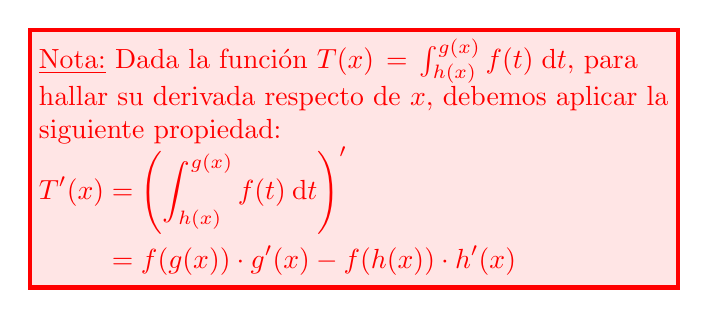
\begin{tikzpicture}[baseline=(current bounding box.center)]
                  \node[red,draw=red,fill=red!10,line width=1.5pt,text width=8cm] {\underline{Nota:} Dada la función $T(x)=\int_{h(x)}^{g(x)}f(t)\dt$, para hallar su derivada respecto de $x$, debemos aplicar la siguiente propiedad: 
                        
                        $ \begin{aligned}
                              T'(x)&=\left(\int_{h(x)}^{g(x)}f(t)\dt\right)'\\
                              &=f(g(x))\cdot g'(x)-f(h(x))\cdot h'(x)
                        \end{aligned}$};
            \end{tikzpicture}
      \end{wrapfigure}
      
      $\db{F(x)=\int_{y}^{\left(\int_1^x\sin^3(t)\dt\right)}\dfrac{1}{1+\sin^6(t)+t^2}\dt}$
      
      $F'(x)=\dfrac{1}{1+\sin^6\left(\int_1^x\sin^3(t)\dt\right)+\left(\int_1^x\sin^3(t)\dt\right)^2}\cdot\left(\int_1^x\sin^3(t)\dt\right)'-\cancel{\dfrac{1}{1+\sin^6(y)+y^2}\cdot0}=\dfrac{1}{1+\sin^6\left(\int_1^x\sin^3(t)\dt\right)+\left(\int_{1}^{x}\sin^3(t)\dt\right)^2}\cdot\left[\sin^3(x)\cdot1-\cancel{\sin^3(1)\cdot0}\right]$
      
      $\bboxed{F'(x)=\dfrac{\sin^3(x)}{1+\sin^6\left(\int_1^x\sin^3(t)\dt\right)+\left(\int_{1}^{x}\sin^3(t)\dt\right)^2}}$
\end{minipage}
\item \lb{Si $f$ es continua en $[0,1]$, calcule $\lim_{x\to0^+}x\int_x^1\dfrac{f(t)}{t}\dt$.}

$\lim_{x\to0^+}x\int_x^1\dfrac{f(t)}{t}\dt=(0\cdot\infty)=\lim_{x\to0^+}\dfrac{\int_x^1\frac{f(t)}{t}\dt}{\frac{1}{x}}=\left(\dfrac{\infty}{\infty}\right)=\{\text{L'Hôpital}\}=\lim_{t\to0^+}\dfrac{\cancel{\frac{f(1)}{1}\cdot0}-\frac{f(x)}{x}\cdot1}{-\frac{1}{x^2}}=\lim_{x\to0^+}\dfrac{\frac{f(x)}{\cancel{x}}}{\frac{1}{x^{\cancel{2}}}}=\lim_{x\to0^+}xf(x)=\{\lim_{x\to0^+}f(x)=f(0)\}=0\cdot f(0)=\bboxed{0}$
\item \lb{Calcular la siguiente integral impropia: \[ \int_{1}^{+\infty}\dfrac{1}{x^3}\dx \]}

$\begin{array}{l}
      \int_{1}^{+\infty}\dfrac{1}{x^3}\dx=\lim_{t\to+\infty}\lbb{\int_{1}^{t}\dfrac{1}{x^3}\dx}{I_1}=\lim_{t\to+\infty}\left(\tozero{\dfrac{-1}{2t^2}}+\dfrac{1}{2}\right)=\dfrac{1}{2}\\
      \lb{I_1=}\int_{1}^{t}x^{-3}\dx=\left[\dfrac{x^{-2}}{-2}\right]_1^t=\left[\dfrac{-1}{2x^2}\right]_1^t=\dfrac{-1}{2t^2}+\dfrac{1}{2}
\end{array}$

Por lo tanto tenemos que la integral es convergente y su valor es: \[ \bboxed{\int_1^{+\infty}\dfrac{1}{x^3}\dx=\dfrac{1}{2}} \]
\item \lb{Calcular la siguiente integral impropia: \[ \int_{0}^{1}\dfrac{1}{\sqrt{x}}\dx \]}

Estamos ante una integral impropia de 2ª especie: \[ \begin{array}{l}
      \int_0^1\dfrac{1}{\sqrt{x}}\dx=\lim_{t\to0^+}\lbb{\int_t^1\dfrac{1}{\sqrt{x}}\dx}{I_1}=\lim_{t\to0^+}(2-\tozero{2\sqrt{t}})=2\\
      \lb{I_1}=\int_{t}^{1}\dfrac{1}{\sqrt{x}}\dx=\int_t^1x^{-\frac{1}{2}}\dx=\left[\dfrac{x^{\frac{1}{2}}}{\frac{1}{2}}\right]_t^1=\left[2\sqrt{x}\right]_t^1=2-2\sqrt{t}
\end{array} \]
Por lo tanto, la integral es convergente, y su valor viene dado por: \[ \bboxed{\int_0^1\dfrac{1}{\sqrt{x}}\dx=2} \]
\item \lb{Calcula:}

$\begin{array}{l}
      \db{\int_{1}^{+\infty}\dfrac{1}{x(x+1)}\dx=}\lim_{t\to+\infty}\lbb{\int_1^t\dfrac{1}{x(x+1)}\dx}{I_1}=\lb{(\ast)}\\
      \begin{aligned}
            \lb{I_1=}\int_1^t\dfrac{1}{x(x+1)}\dx=\int_1^t\dfrac{1}{x}-\dfrac{1}{x+1}\dx=\left[\ln(x)-\ln(x+1)\right]_1^t&=\ln(t)-\ln(t+1)-\tozero{\ln(1)}+\ln(2)\\
            &=\ln\left(\dfrac{t}{t+1}\right)+\ln(2)
      \end{aligned}\\
      \dfrac{1}{x(x+1)}=\dfrac{A}{x}+\dfrac{B}{x+1}=\dfrac{A(x+1)+Bx}{x(x+1)}\\
      1=A(x+1)+Bx\begin{cases}
            \text{Si }x=0\longrightarrow A=1\\
            \text{Si }x=-1\longrightarrow B=-1
      \end{cases}\quad\dfrac{1}{x(x+1)}=\dfrac{1}{x}-\dfrac{1}{x+1}\\
      \lb{(\ast)=}\lim_{t\to+\infty}\left[\ln\left(\dfrac{t}{t+1}\right)+\ln(2)\right]=\tozero{\ln(1)}+\ln(2)=\ln(2)\\
      \lim_{t\to+\infty}\dfrac{t}{t+1}=\left(\dfrac{\infty}{\infty}\right)=\{\text{L'Hôpital}\}=\lim_{t\to+\infty}\dfrac{1}{1}=1
\end{array}$

La integral impropia es convergente y su valor es: \[ \bboxed{\int_{1}^{+\infty}\dfrac{1}{x(x+)}\dx=\ln(2)} \]
\item \lb{Calcula:}

$\db{\int_0^1\dfrac{e^x}{\sqrt{e^x-1}}\dx}$

Estamos ante una integral impropia de 2ª especie: \[ \int_0^1\dfrac{e^x}{\sqrt{e^x-1}}\dx=\lim_{t\to0^+}\lbb{\int_t^1\dfrac{e^x}{\sqrt{e^x-}}\dx}{I_1}=\lb{(\ast)} \]Vamos a hacer primero la primitiva: \[ \begin{array}{l}
      \int\dfrac{e^x}{\sqrt{e^x-1}}\dx=\left\{\begin{array}{l}
      e^x-1=T\\
      e^x\dx=\dt
\end{array}\right\}=\int\dfrac{1}{\sqrt{t}}\dt=\int t^{-\frac{1}{2}}\dt=\dfrac{t^{\frac{1}{2}}}{\frac{1}{2}}=2\sqrt{t}=2\sqrt{e^x-1}\\
\lb{(\ast)=}\lim_{t\to0^+}\left[2\sqrt{e^x-1}\right]_t^1=\lim_{t\to0^+}(2\sqrt{e-1}-\tozero{2\sqrt{e^t-1}})=2\sqrt{e-1}
\end{array} \] Por lo tanto, la integral es convergente y su valor es: \[ \bboxed{\int_0^1\dfrac{e^x}{\sqrt{e^x-1}}\dx=2\sqrt{e-1}} \]
\item \lb{Calcula:}

$\db{\int_1^1\ln(x)\dx)}\lim_{t\to0^+}\int_{t}^{1}\ln(x)\dx=\lb{(\ast)}$

Calcularemos la primitiva: \[ \begin{array}{l}
      \int\ln(x)\dx)\left\{\begin{array}{ll}
            u=\ln(x) & \du=\dfrac{1}{x}\dx\\
            \dv=1\dx & v=x
      \end{array}\right\}=x\ln(x)-\int \cancel{x}\cdot\dfrac{1}{\cancel{x}}\dx=x\ln(x)-x\\
      \lb{(\ast)=\lim_{t\to0^+}\left[x\ln(x)-x\right]_t^1=\lim_{t\to0^+}(\tozero{1\cdot\ln(1)}-1-\lbb{t\ln(t)}{L_1}+\tozero{t})}=\bboxed{-1}\\
      \lb{L_1=}\lim_{t\to0^+}t\ln(t)=(0\cdot\infty)=\lim_{t\to0^+}\dfrac{\ln(t)}{\frac{1}{t}}=\left(\dfrac{\infty}{\infty}\right)=\{\text{L'Hôpital}\}=\lim_{t\to0^+}\dfrac{\frac{1}{t}}{-\frac{1}{t^2}}=\lim_{t\to0^+}\dfrac{-t^{\cancel{2}}}{\cancel{t}}=\lim_{t\to0^+}(-t)=0
\end{array} \]
Por lo tanto es una integral convergente y su valor es:\[ \bboxed{\int_0^1\ln(x)\dx=-1} \]
\item \lb{Calcula:}

$\db{\int_0^{\frac{1}{e}}\dfrac{1}{\left(\ln(x)\right)^2x}}$

\begin{center}
      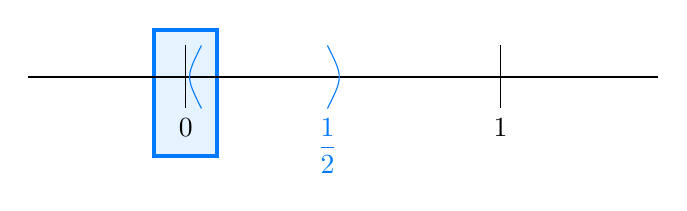
\begin{tikzpicture}[scale=4]
            \draw[draw=lightblue,fill=lightblue!10,line width=1.5] (-0.1,0.15) rectangle (0.1,-0.25);
            \draw (-0.5,0) -- (1.5,0);
            \foreach \x in {0,1}{
            \draw (\x,0.1) -- (\x,-0.1) node[below] {$\x$};
            }
            \draw[lightblue] (0.05,0.1) .. controls (0,0) .. (0.05,-0.1);
            \draw[lightblue] (0.45,0.1) .. controls (0.5,0) .. (0.45,-0.1) node[below] {$\dfrac{1}{2}$};
             
      \end{tikzpicture}
\end{center}
\[\int_0^{\frac{1}{e}}\dfrac{1}{(\ln(x))^2x}\dx=\lim_{t\to0^+}\int_{t}^{\frac{1}{e}}\dfrac{1}{(\ln(x))^2x}\dx=\lb{(\ast)}\]Hacemos la primitiva a parte: \[ \begin{array}{l}
      \int\dfrac{1}{(\ln(x))^2\cdot x}\dx=\int\dfrac{1}{(\ln(x))^2}\cdot\dfrac{1}{x}\dx=\left\{\begin{array}{l}
            \ln(x)=u\\
            \dfrac{1}{x}\dx=\du
      \end{array}\right\}=\int\dfrac{1}{u^2}\du=\int u^{-2}\du=\dfrac{u^{-1}}{-1}=-\dfrac{1}{u}=-\dfrac{1}{\ln(x)}\\
      \lb{(\ast)=}\lim_{t\to0^+}\left[-\dfrac{1}{\ln(x)}\right]_{t}^{\frac{1}{e}}=\lim_{t\to0^+}\left(-\dfrac{1}{\cancel{\ln}(\cancel{e})^{-1}}+\tozero{\dfrac{1}{\ln(t)}}~~~\right)=\left\{\ln(e)^{-1}=(-1)\lbb{\ln(e)}{1}=-1\right\}=1
\end{array} \]La integral impropia es convergente y su valor es: \[ \bboxed{\int_{0}^{1}\dfrac{1}{(\ln(x))^2x}\dx=1} \]
\item \lb{Calcular la integral:}

$\db{\int_{1}^{+\infty}\dfrac{1}{1+x^2}\dx=}\lim_{t\to+\infty}\dfrac{1}{t}\dfrac{1}{1+x^2}\dx=\lim_{t\to+\infty}\left[\arctan(x)\right]_1^t=\lim_{t\to+\infty}\left[\arctan(t)-\arctan(1)\right]=\underset{\begin{subarray}{c}
            \rotatebox{90}{=}\\
            \frac{\pi}{2}
\end{subarray}}{\arctan(+\infty)}-\underset{\begin{subarray}{c}
\rotatebox{90}{=}
\end{subarray}}{\frac{\pi}{4}}=\dfrac{\pi}{2}-\dfrac{\pi}{4}=\bboxed{\dfrac{\pi}{4}}$

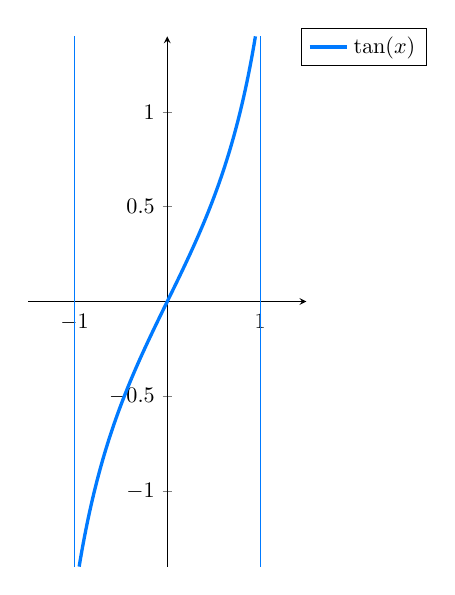
\begin{tikzpicture}[scale=0.8, baseline=(current bounding box.center)]% function
      \begin{axis}[domain=-0.95:0.95,
            samples=400,
            axis lines=center,height=10cm,width=6cm, xmin=-1.5, xmax=1.5, legend style={anchor=west}]
            \addplot[lightblue,line width=1.5, mark=none] {tan(deg(x))};
            \addlegendentry{$\tan(x)$}
            \draw[lightblue] (axis cs:1,1.5) -- (axis cs:1,-1.5);
            \draw[lightblue] (axis cs:-1,1.5) -- (axis cs:-1,-1.5);
      \end{axis}
\end{tikzpicture}$\qquad\lb{\begin{array}{l}
      \tan(0)=0\\
      \tan\left(\dfrac{\pi}{4}\right)=1\\
      \tan\left(\dfrac{\pi}{6}\right)=\dfrac{1}{\sqrt{3}}\\
      \tan\left(\dfrac{\pi}{3}\right)=\sqrt{3}\\
      \tan\left(-\dfrac{\pi}{4}\right)=-1\\
      \tan\left(-\dfrac{\pi}{6}\right)=-\dfrac{1}{\sqrt{3}}\\
      \tan\left(-\dfrac{\pi}{3}\right)=-\sqrt{3}\\
      \tan\left(\dfrac{\pi}{2}^{-}\right)=+\infty\\
      \tan\left(\dfrac{\pi}{2}^{+}\right)=-\infty\\
      \end{array}}$
\item \lb{Calcular la siguiente integral}

$\db{\int\dfrac{1}{(x-1)(x^2+2)}\dx=}\lb{(\ast)}$

Aplicaremos para empezar, separación por fracciones simples: 

$\begin{array}{l}
      \dfrac{1}{(x-1)(x^2+2)}=\dfrac{A}{x-1}+\dfrac{Bx+C}{x^2+2}=\dfrac{A(x^2+2)+(x-1)}(Bx+C){(x-1)(x^2+2)}\\
      1=A(x^2+2)+(x-1)(Bx+C)\\
      \begin{array}{l}
            \text{Si }x=1\longrightarrow 3A=1\longrightarrow\bboxed{A=\dfrac{1}{3}}\\
            \text{Si }x=0\longrightarrow1=\dfrac{2}{3}+(-1)C\longrightarrow\bboxed{C=-\dfrac{1}{3}}\\
            \text{Si }x=-1\longrightarrow\cancel{1})=\cancel{1}+(-2)\left(-B-\dfrac{1}{3}\right)\longrightarrow\bboxed{B=-\dfrac{1}{3}}
      \end{array}\dfrac{1}{(x-1)(x^2+2)}=\dfrac{1}{3}\cdot\dfrac{1}{x-1}+\dfrac{-\frac{1}{3}x-\frac{1}{3}}{x^2+2}\\
      \lb{(\ast)=}\int\dfrac{1}{3}\cdot\dfrac{1}{x-1}+\dfrac{-\frac{1}{3}x-\frac{1}{3}}{x^2+2}\dx=\dfrac{1}{3}\lbb{\int\dfrac{1}{x-1}\dx}{I_1}-\dfrac{1}{3}\dbb{\int\dfrac{x}{x^2+2}\dx}{I_2}-\dfrac{1}{3}\rb{\int\dfrac{1}{x^2+2}\dx}{I_3}=\lb{(\ast\ast)}\\
      \lb{I_1=}\int\dfrac{1}{x-1}\dx=\log|x-1|\\
      \db{I_2=}\int\dfrac{x}{x^2+2}\dx=\dfrac{1}{2}\int\dfrac{2x}{x^2+2}\dx=\left\{\begin{array}{l}
            x^2+2=t\\
            2x\dx=\dt
      \end{array}\right\}=\dfrac{1}{2}\int\dfrac{1}{t}\dt=\dfrac{1}{2}\ln|t|=\dfrac{1}{2}\ln|x^2+2|\\
      \begin{aligned}
            \rc{I_3}&\rc{=}\int\dfrac{1}{x^2+2}\dx=\int\dfrac{\frac{1}{2}}{\frac{x^2}{2}+1}\dx=\dfrac{1}{2}\int\dfrac{1}{\left(\frac{x}{\sqrt{2}}\right)^2+1}\dx=\dfrac{\sqrt{2}}{2}\int\dfrac{\frac{1}{\sqrt{2}}}{\left(\frac{x}{\sqrt{2}}\right)^2+1}\dx=\left\{\begin{array}{l}
            \dfrac{x}{\sqrt{2}}=t\\
            \dfrac{1}{\sqrt{2}}\dx=\dt
      \end{array}\right\}\\
      &=\dfrac{\sqrt{2}}{2}\int\dfrac{1}{t^2+1}\dt=\dfrac{\sqrt{2}}{2}\arctan(t)=\dfrac{\sqrt{2}}{2}\arctan\left(\dfrac{x}{\sqrt{2}}\right)
      \end{aligned}\\
      \lb{(\ast\ast)=}\bboxed{\dfrac{1}{3}\log|x-1|-\dfrac{1}{6}\ln|x^2+2|-\dfrac{\sqrt{2}}{6}\arctan\left(\dfrac{x}{\sqrt{2}}\right)+\mathrm{C}}
\end{array}$
\item \lb{Calcular la siguiente integral:}

$\db{\int\sin^2(x)\cdot\cos^2(x)\dx=}\left\{\begin{array}{l}
      \sin(2x)=2\sin(x)\cos(x)\\
      \sin^2(2x)=4\sin^2(x)\cos^2(x)
\end{array}\right\}=\int\dfrac{1}{4}\sin^2(2x)\dx=\left\{\sin^2(x)=\dfrac{1-\cos^2(x)}{2}\right\}=\dfrac{1}{4}\int\dfrac{1-\cos(4x)}{2}\dx=\dfrac{1}{8}\left(x-\dfrac{\sin(4x)}{4}\right)+\mathrm{C}=\bboxed{\dfrac{1}{8}x-\dfrac{1}{32}\sin(4x)+\mathrm{C}}$
\pagebreak
\item \lb{Calcular la siguiente integral:}

$\begin{aligned}
      \db{\int x^2\sin(3x)\dx}&\db{=}\left\{\begin{array}{ll}
      u=x^2 & \du=2x\\
      \dv=\sin(3x)\dx & v=-\dfrac{\cos(3x)}{3}
\end{array}\right\}=-\dfrac{x^2}{3}\cos(3x)+\dfrac{2}{3}\int x\cos(3x)\dx\\
&=\left\{\begin{array}{ll}
u=x & \du=\dx\\
\dv=\cos(3x)\dx& v=\dfrac{\sin(3x)}{3}
\end{array}\right\}=-\dfrac{x^2}{3}\cos(3x)+\dfrac{2}{3}\left[x\dfrac{\sin(3x)}{3}-\int\dfrac{\sin(3x)}{3}\dx\right]\\
&=-\dfrac{1}{3}x^2\cos(3x)+\dfrac{2}{9}x\sin(3x)-\dfrac{2}{9}\int\sin(3x)\dx\\
&=\bboxed{-\dfrac{1}{3}x^2\cos(3x)+\dfrac{2}{9}x\sin(3x)+\dfrac{2}{27}\cos(3x)+\mathrm{C}}
\end{aligned}$
\item \lb{Calcular la siguiente integral:}

\begin{minipage}[l]{\textwidth}
      \begin{wrapfigure}{r}{0.3\textwidth}
            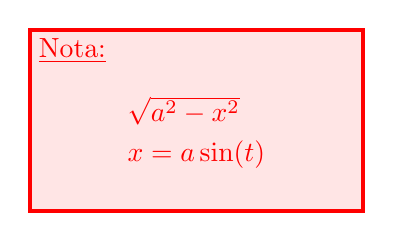
\begin{tikzpicture}[baseline=(current bounding box.center)]
                  \node[red,draw=red,fill=red!10,line width=1.5pt,text width=4cm] {\underline{Nota:} \[ \begin{array}{l}
                              \sqrt{a^2-x^2}\\
                              x=a\sin(t)
                        \end{array} \]};
            \end{tikzpicture}
      \end{wrapfigure}
      
      $\db{\int\sqrt{4-x^2}\dx=}\int\sqrt{4-\sin(t)}\dt=\left\{\begin{array}{l}
                  x=2\sin(t)\\
                  \dx=2\cos(t)\dt
            \end{array}\right\}=\int\sqrt{4-(2\sin(t))^2}\cdot2\cos(t)\dt=\int\sqrt{4-4\sin^2(t)}\cdot2\cos(t)\dt=\int\underset{\begin{subarray}{c}
                  \rotatebox{90}{=}\\
                  \cos^2(t)
                  \end{subarray}}{\sqrt{4(1-\sin^2(t))}}\cdot2\cos(t)\dt=4\int\cos^2(t)\dt=4\int\dfrac{1+\cos(2t)}{2}\dt=2\left[t+\dfrac{\sin(2t)}{2}\right]+\mathrm{C}=2t+2\sin(t)\cos(t)+\mathrm{C}=\lb{(\ast)}$
\end{minipage}

$\begin{array}{l}
      x=2\sin(t)\longrightarrow\bboxed{\sin(t)=\dfrac{x}{2}}\longrightarrow\bboxed{t=\arcsin\left(\dfrac{x}{2}\right)}\\
      \begin{aligned}
            \cos^2(t)+\sin^2(t)=1&\longrightarrow\cos(t)=\sqrt{1-\sin^2(t)}=\sqrt{1-\left(\dfrac{x}{2}\right)^2}=\sqrt{1-\dfrac{x^2}{4}}=\dfrac{\sqrt{4-x^2}}{2}\\
            &\longrightarrow\bboxed{\cos(t)=\dfrac{1}{2}\sqrt{4-x^2}}
      \end{aligned}\\
      \\
      \lb{(\ast)=}2\arcsin\left(\dfrac{x}{2}\right)+\cancel{2}\cdot\dfrac{x}{\cancel{2}}\cdot\dfrac{1}{2}\sqrt{4-x^2}+\mathrm{C}=\bboxed{2\arcsin\left(\dfrac{x}{2}\right)+\dfrac{1}{2}\sqrt{4-x^2}+\mathrm{C}}
\end{array}$

\pagebreak

\item \lb{Calcule $f(4)$ si \[ \int_{0}^{x^2}f(t)\dt=x\cos(\pi x) \]}

\begin{minipage}[l]{\textwidth}
      \begin{wrapfigure}{r}{0.45\textwidth}
            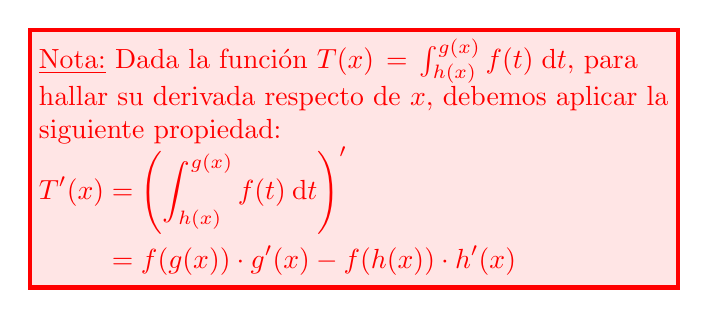
\begin{tikzpicture}[baseline=(current bounding box.center)]
                  \node[red,draw=red,fill=red!10,line width=1.5pt,text width=8cm] {\underline{Nota:} Dada la función $T(x)=\int_{h(x)}^{g(x)}f(t)\dt$, para hallar su derivada respecto de $x$, debemos aplicar la siguiente propiedad: 
                        
                        $ \begin{aligned}
                              T'(x)&=\left(\int_{h(x)}^{g(x)}f(t)\dt\right)'\\
                              &=f(g(x))\cdot g'(x)-f(h(x))\cdot h'(x)
                        \end{aligned}$};
            \end{tikzpicture}
      \end{wrapfigure}
      
      Lo que vamos a hacer es derivar esta ecuación: 
      
      $\left(\int_{0}^{x^2}f(t)\dt\right)'=f(x^2)\cdot2x-\cancel{f(0)\cdot0}=2xf(x^2)$
      
      $(x\cos(\pi x))'=1\cos(\pi x)+x\cdot(-\sin(\pi x))\cdot\pi=\cos(\pi x)-x\sin(\pi x)$
      
      Igualando: $2xf(x^2)=\cos(\pi x)-x\sin(\pi x)$
      
      $\bboxed{f(x^2)=\dfrac{1}{2x}\left[\cos(\pi x)-x\sin(\pi x)\right]}$
      
      $f(4)=f(2^2)=\{x=2\}=\dfrac{1}{4}[\underset{\begin{subarray}{c}
                  \rotatebox{90}{=}\\
                  1
      \end{subarray}}{\cos(2\pi)}-\tozero{2\sin(2\pi)}]\longrightarrow\bboxed{f(4)=\dfrac{1}{4}}$
\end{minipage}
\end{enumerate}
\end{document}

\begin{minipage}[l]{\textwidth}
      \begin{wrapfigure}{r}{0.35\textwidth}
            
\begin{tikzpicture}[baseline=(current bounding box.center)]
                  \node[red,draw=red,fill=red!10,line width=1.5pt,text width=6cm] {};
            \end{tikzpicture}
      \end{wrapfigure}
\end{minipage}